\section{Verification, reproducibility, and remaining scope}
\label{sec:verification}

\subsection{What was checked exactly}

The general assertions are proved in the preceding sections. The finite
checks test independent formulations and boundary cases; they do not
establish the theorems by extrapolation. All arithmetic in the substantive
verification scripts is exact.

\begin{center}
\small
\begin{tabularx}{\linewidth}{@{}L{0.34\linewidth}YL{0.18\linewidth}@{}}
\toprule
Check & Scope & Outcome\\
\midrule
Exhaustive cubic packet comparison &
$r=1$, $k=1,\ldots,8$; $r=2$, $k=1,\ldots,6$;
$r=3$, $k=1,2,3$; $r=4$, $k=1,2$ &
17\,735\,976 pairs; all agree\\[3pt]
Extremizer structure & Translation periods and quotient forms, including
repeated saturated entries & 5285 extremizers checked\\[3pt]
Eisenstein local cost & Nonzero zero-sum triples of positive mass at most
300 & 270\,900 triples checked\\[3pt]
Sharp constructions and Fourier norms & Two- and four-coset constructions
through rank six & 36 constructions checked\\[3pt]
Independent cubic implementation & Separate local multiplicity enumeration
in 13 small parameter cases & 1\,036\,722 pairs; all agree\\[3pt]
Unequal branch recovery & 625 exhaustive profiles, 120 seeded finite-field
examples, two displayed examples & 747 profiles checked\\[3pt]
Direct branch matrix ranks & Compare unresolved-jet dimensions using exact
finite-field elimination & 2996 comparisons pass\\[3pt]
Pruning and saturation & Compare tree recursion with all branch subsets;
check the componentwise distance criterion & 2996 checks each pass\\
\bottomrule
\end{tabularx}
\end{center}

The independent cubic implementation does not use Eisenstein valuations
or Reed--Muller weights. It compares the three local-root multiplicities
directly, so its agreement with the density theorem tests a different
description. The principal implementation also checks the proposed
extremizer families using their translation stabilizers. Structural checks
were capped at 500 extremal pairs per parameter case; the minimum-density
comparison itself includes every pair in the displayed ranges.

For branches, direct expansion and row reduction determine the ambiguity
of the target jet after allowing unrestricted higher terms up to the
finite observation cutoff. A separate contact-tree computation is checked
against enumeration of all retained subsets. The finite-field runs also
check 1423 successful sparse recovery certificates. They use fixed seed
\code{20261127}; no random floating-point linear algebra is involved.

An independent agent reviewed both mathematical arguments adversarially.
The reviews are included in the archive. One wording error was corrected:
branch ambiguity witnesses have small $Y$-degree and small total
\emph{order}; their total degree need not be small. This matters when a
branch contains high powers of $X$. The final manuscript states the
correct property and explains finite polynomial truncation.

\begin{figure}[htbp]
\centering
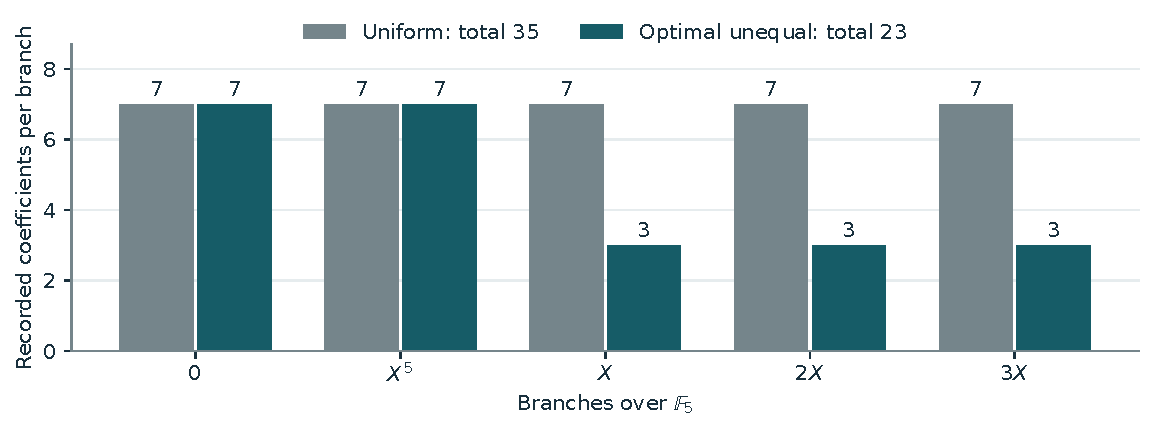
\includegraphics[width=0.92\linewidth]{figures/precision_budget.pdf}
\caption{The sharp five-branch allocation example over $\F_5$.
Both allocations recover the order-three jet despite one arbitrary
corrupted record. The unequal profile uses 23 coefficients; every uniform
profile with the same guarantee uses at least 35.}
\end{figure}

\subsection{Rebuilding and interpreting the artifacts}

The archive contains the main \code{report.tex}, its chapter sources,
compiled \code{report.pdf}, bibliography, verification code, JSON outputs,
figure sources and outputs, provenance, and proof-review notes.
The \code{Makefile} provides the following targets:
\begin{itemize}
\item \code{make pdf}: compile the manuscript with \code{latexmk};
\item \code{make verify}: rerun the exact mathematical checks;
\item \code{make figures}: regenerate publication figures from the stated
formulas and recorded exact examples;
\item \code{make source-audit SOURCE=/path/to/ProveIt}: rerun the local
source scan against a separately obtained checkout.
\end{itemize}
Both cubic verifiers use NumPy; the branch verifier uses only the Python
standard library. The delivered results record the
actual test environment. A full upstream source checkout and third-party
papers are not copied into the archive. Pinned links and a file manifest
identify what was read. Rebuilding the new manuscript or rerunning its
finite checks does not build the upstream Lean project.

\subsection{Novelty assessment and boundaries}

The exact cubic extremal function and its complete equality classification
were not found in the supplied article, its relevant recent reports, or
the seven incoming ZIP reports at the pinned revision. The proof directly
extends the article's quadratic Fourier/valuation approach. The new
features are the two Eisenstein valuation costs, the parity obstruction to
an even minimum support, and the resulting sharp packet classifications.
Known coding theorems are explicitly cited, and the generic
$k^2\log^2 Q$ detection scale is not claimed as new.

Targeted primary-literature searches covered cubic-character matching,
integral ternary Fourier uncertainty, and finite-group character matching.
Walji's matching-density work and Martin--Walji's character comparison
results address adjacent representation-theoretic questions
\cite{walji2016,martinwalji2017}; they do not state the reducible cubic
packet classification proved here. The second extension explicitly
credits weighted greedy selection to established work
\cite{grinbergpetrov}. A search that does not find an exact predecessor
does not establish worldwide priority. These results should be treated
as proved research contributions relative to the supplied collection,
with priority subject to further expert literature review.

The following tasks are not settled here: the full cubic nonextremal
density spectrum, the matching problem for every odd prime exponent,
mixed coefficient rings $\mathcal O/\pi^r$ with $r>1$, and a fast
error-location decoder. The dynamic program computes the exact
branch distance and extremal deletion set; it does not by itself locate
corrupted records from arbitrary received values.

Finally, none of the new theorems is a Lean-certified extension of the
vendor package. The document gives mathematical proofs and reproducible
exact checks. The appendix describes how a future formalization can be
separated into finite algebraic work and the single analytic interface.
